There are two main ways of including diagrams in an entry: inline and externally.

Inline diagrams are generated by code included directly in the TeX document. They are rendered using specific packages such as \texttt{xypic}, \texttt{pstricks}, etc. However, some of them only work with PostScript output and cannot be compiled directly with PDFLaTeX or PDFTeX.

External figures are usually EPS (Encapsulated PostScript), PostScript, or PDF files, which can be generated with a large number of programs (see below). Once created, they should be uploaded to the article's PlanetMath filebox, along with the source (for example, the FIG file if XFig was the drawing program). Including the source alleviates concerns about compliance with the FDL license, and is just the ``right thing'' to do.

\subsection*{External graphics.}
In order to use graphics, the proper packages need to be loaded. In the case of external images we add the following line to the \emph{Preamble} section of the entry:
\begin{quote}
\begin{Verbatim}
\usepackage{graphicx}
\end{Verbatim}
\end{quote}

Now, suppose we have uploaded the file \texttt{pmlogo.eps} on the filebox at the bottom of the editing dialog. Whenever we wanted to include the picture we add the lines:

\begin{Verbatim}
\begin{center}

\includegraphics{./inputs/pmlogo}
\end{center}
\end{Verbatim}


The centering is optional, and notice how we omitted the extension. The result after rendering is
\begin{center}

\includegraphics{./inputs/pmlogo}
\end{center}
Notice the image is a bit blurry, the reason being that it is not a vector-based graphic, but a raster one (something to be avoided). See \ref{gfxformats} for information.

Now, \texttt{includegraphics} has several optional parameters that affect its output. We can scale with \texttt{scale=}\emph{x}:

\begin{quote}
\begin{verbatim}

\includegraphics[scale=0.5]{pmlogo}
\end{verbatim}
\end{quote}

Since \texttt{scale=0.5}, the resulting size image is halved:

\begin{center}

\includegraphics[scale=0.5]{./inputs/pmlogo}
\end{center}

Sometimes you need to rotate your graphics. You can do that with the \texttt{angle=}\emph{x} option, where \emph{x} is the angle in degree by which the image is rotated counterclockwise.

\begin{quote}
\begin{verbatim}

\includegraphics[scale=0.3,angle=90]{pmlogo}
\end{verbatim}
\end{quote}

\begin{center}

\includegraphics[scale=0.3,angle=90]{./inputs/pmlogo}
\end{center}

\subsubsection*{Placing labels and numbering}
Perhaps you want to put some lines of text and a number under your image (this is generally a good idea). To achieve this use the following:

\begin{quote}
\begin{verbatim}
\begin{figure}[h] %The [h] puts the figure to the actual position
\begin{centering} %This centers the image (not necessary but nicer)

\includegraphics{pmlogo} %Of course you can still scale the image
\caption{The PlanetMath logo} %This creates the image text and a number
\end{centering}
\end{figure}
\end{verbatim}
\end{quote}

Now you get this result:
\begin{figure}[h]
\begin{centering}

\includegraphics{./inputs/pmlogo}
\caption{The PlanetMath logo}
\end{centering}
\end{figure}

\subsection*{Creating your graphics.}
\subsubsection*{Issues.}
Mention the raster vs vector issue again.
\subsubsection*{xfig}
\subsubsection*{pstricks}
One of the best ways to create graphics is using PSTricks, which is a package to do PostScript inside LaTeX. PSTricks documentation is freely available on the Web; a good reference is at
\htmladdnormallink{http://www.dante.de/CTAN/graphics/pstricks/base/doc/pstricks-doc.pdf}{http://www.dante.de/CTAN/graphics/pstricks/base/doc/pstricks-doc.pdf}

\textbf{Advantages.}
\begin{itemize}
\item It is not dependent on the operating system nor on having programs other than a decent TeX system (if you use the PlanetMath rendering engine and code directly on the entry, you don't even need that), and thus graphics can be created on Windows, Linux, etc.
\item The graphics obtained are of very high quality, and if the graphics are exported with \texttt{dvips}, the result are standards compliant EPS files which can be used without problem with LaTeX and LaTeX2HTML.
\item There are many specialized subpackages for doing common drawings in a simpler way (plotting mathematical functions, geometric shapes, etc.).
\end{itemize}

\textbf{Disadvantages.}
\begin{itemize}
\item It can be a little intimidating when approached for the first time (like when approaching LaTeX for the first time. ;-)
\item When used directly on PlanetMath, there are several quirks not to be forgotten.
\item PSTricks uses PostScript special commands, so will not support generation of PDF files. This can be remedied by using the \texttt{pst-pdf} package. This is not an issue for use of PSTricks within PlanetMath, but it may be an issue for you if you are developing your pages offline with your own TeX system.
\end{itemize}

\subsubsection{PSTricks useful examples.}
Here are two examples of the use of PSTricks on PlanetMath, with comments. The first is from the entry \texttt{NormalLine} (available at \\ \htmladdnormallink{http://planetmath.org/encyclopedia/NormalLine.html}{http://planetmath.org/encyclopedia/NormalLine.html}):

\begin{Verbatim}
\begin{center}
% Set the lower left of the image at (-2,-1) and the upper right at (2,4)
\begin{pspicture}(-2,-1)(2,4)
% Draw a parabola through (2,4) with a minimum (or maximum) at (0,0)
\parabola{-}(2,4)(0,0)
% Draw a red line between the given points
\psline[linecolor=red](0,-1)(2,3)
% Draw a blue line between the given points
\psline[linecolor=blue](-2,2.5)(2,0.5)
% Put a large dot at (1,1)
\psdot(1,1)
% and label the dot
\rput[b](0.9,1.2){$P$}
% Finally, mark the right angle between the tangent and normal lines
\psline[linewidth=0.2pt](0.9,0.8)(1.1,0.7)
\psline[linewidth=0.2pt](1.1,0.7)(1.2,0.9)
\end{pspicture}
\end{center}
\end{Verbatim}

The second example is from \texttt{GarfieldsProofOfPythagoreanTheorem} (available at \htmladdnormallink{http://planetmath.org/encyclopedia/GarfieldsProofOfPythagoreanTheorem.html} {http://planetmath.org/encyclopedia/GarfieldsProofOfPythagoreanTheorem.html}).

First, in the preamble, we have

\begin{Verbatim}
\usepackage{pst-plot}
\usepackage{psfrag}

% define commands here
\newrgbcolor{LightYellow}{1 1 0.7}
\newrgbcolor{LightBlue}{0.7 1 1}
\newrgbcolor{LightRed}{1 0.7 0.7}
\end{Verbatim}
This includes the \texttt{ps-plot} and \texttt{psfrag} packages. (For some reason, none of this works if \texttt{pstricks} is included instead, or even in addition.) Then, three custom colors are defined for later use.

The entry itself contains
\begin{Verbatim}
\begin{center}
\begin{pspicture}(-.5,-.5)(7.5,4.5)
% Filled objects should be filled with the solid color
\psset{fillstyle=solid}
% Create three contiguous right triangles, differently filled
\pspolygon[fillcolor=LightYellow](0,0)(3,0)(0,4)
\pspolygon[fillcolor=LightBlue](3,0)(7,0)(7,3)
\pspolygon[fillcolor=LightRed](3,0)(7,3)(0,4)
% Label the sides of each
\rput(-0.25,2){b}
\rput(1.5,-0.25){a}
\rput(5,-0.25){b}
\rput(7.25,1.6){a}
\rput(1.75,2){c}
\rput(4.75,1.5){c}
% Draw three right angles. Note that while psline, used in the
% previous example, allows you to draw lines between a list of
% coordinates, to bend the line, and to attach arrowheads, qline is a
% simpler form that just draws a line between one pair of coordinates.
\qline(0,0.25)(.25,.25)
\qline(.25,.25)(.25,0)
\qline(6.75,0)(6.75,.25)
\qline(6.75,.25)(7,.25)
\qline(3.2,.15)(3.05,.35)
\qline(3.05,.35)(2.85,.2)
\end{pspicture}
\end{center}
\end{Verbatim}

\subsubsection{A reminder.}

Note that diagrams drawn using PSTricks are drawn in the order in which the commands occur. Thus, the last object declared will appear on top. Be sure to always be mindful of this. For example, if you want to plot a point using \texttt{psdot} or \texttt{psdots} and you want to draw a line or curve in any color other than black that passes through that point, you should put the command for drawing the line or curve before the command for plotting the point. Thus, the point will be drawn last and appear totally black rather than having a colored line passing through it.

\subsubsection{PlanetMath and PSTricks}

Due to some technical details, when doing graphics directly on PlanetMath some considerations need to be taken:
\begin{itemize}
\item It seems that the declaration \verb+\usepackage{pstricks}+ must appear relatively early in the preamble (i.e., the fourth line or prior) in order for graphics drawn via PSTricks to display correctly in either viewing mode (html or page images).
\item All pictures are to be done between \verb+\begin{pspicture}(xmin,ymin)(xmax,ymax)+
and \verb+\end{pspicture}+. Here, \verb+(xmin,ymin)+ and \verb+(xmax,ymax)+ specify the lower left and upper right corners of the bounding box of the image. All drawing is with respect to those coordinates, and thus normally has \verb+x+ coordinates between \verb+xmin+ and xmax, and \verb+y+ coordinates between \verb+ymin+ and \verb+ymax+. Drawing outside of the given bounding box is allowed. If you wish to clip the picture to stay within the bounding box, use \verb+pspicture*+.
\item No PSTricks commands can appear outside the previous environment.
\item In normal (that is, outside of PlanetMath) PSTricks usage, you can redefine your units using the \texttt{psset} command. However, since all PSTricks commands in PlanetMath must appear within the \texttt{pspicture} environment, this will not work. Thus if you want to redefine, or stretch/contract, your image, coordinates will need to be manually recalculated.
\item The use of nodes is unsupported. (In particular, this means that the \texttt{pst-eucl} package for geometrical drawings is problematic.)
\item If you look carefully at the two entries given as examples above, you will see that the code given does not exactly match the code in the entry. For example, the \texttt{NormalLine} entry contains the three additional lines
\begin{Verbatim}
\rput[b](-2,4){.}
\rput[b](2,4){.}
\rput[l](-0.05,-1){.}
\end{Verbatim}
These points are drawn here to overcome a bug in PlanetMath in which PSTricks images are clipped to the text only; if lines or polygons go beyond the text, they may be clipped in the result. The \texttt{rput} commands here place unobtrusive dots at the edges of the diagram to force PlanetMath to maintain the desired image boundaries. This bug exists only in HTML mode; page mode displays correctly even without the above workaround.
\end{itemize}
\subsubsection{Exporting PSTricks to EPS}
If you want to be on the side safe, the best way is to export your PSTricks graphic to an EPS, upload it to the entry and use the method outlined at the beggining of the guide. In order to export a PSTricks graphic you need to have dvips installed (it comes with almost all TeX distributions, in particular with TeTeX and MikTeX).

The procedure consists on creating a document that contains only your graphic and nothing more, not even page numbers and headings. Suppose the file is named \verb+onlygraphic.tex+, then after compiling it, run \verb+dvips+ with the following parameters:
\begin{quote}
\begin{verbatim}
dvips -E onlygraphic.dvi -o onlygraphic.eps
\end{verbatim}
\end{quote}

Now the question is, how do one gets a blank file with nothing but the graphic?
Here is a sample file \verb+onlygraphic.tex+ to illustrate the required steps.

\begin{Verbatim}
\documentclass{scrartcl} % It could use article or any base class
\usepackage{pstricks} % Needed to work with PStricks
\usepackage{color} % Will be used to create an invisible box

\begin{document}
\pagestyle{empty} % To supress page numbers and headings
\colorbox{white}{ % Could be replaced by \framebox if
% color package is not available
\begin{pspicture*}(-1,-1)(4,5)
\pspolygon(0,0)(3,0)(3,4) % Code to draw a nice triangle...
\uput[-150](0,0){$A$} % ...label its vertices...
\uput[-30](3,0){$B$}
\uput[90](3,4){$C$}
\psarc(0,0){0.5}{0}{53.13} % ...mark an angle
\uput[45](0.4,0.1){$\alpha$}
\end{pspicture*}
}
\end{document}
\end{Verbatim}

Now, after running \verb+dvips -E onlygraphic.dvi -o RightTriangle.eps+ we can upload \verb+RightTriangle.eps+ to the entry in order to obtain
\begin{Verbatim}
\begin{center}
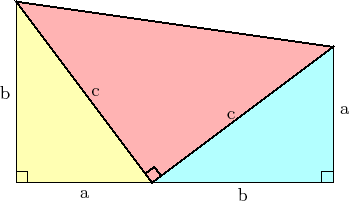
\includegraphics{./inputs/RightTriangle}
\end{center}
\end{Verbatim}
\begin{center}
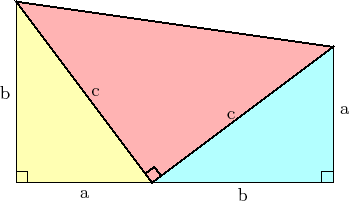
\includegraphics{./inputs/RightTriangle}
\end{center}
\subsubsection{Other details.}
The \verb+pst*+ packages should be loaded the latest on the preamble. Specifically \emph{after} other graphics packages like \verb+graphicx.sty+, \verb+color.sty+ which seem to break \verb+\psgrid+ and other commands.
\subsubsection*{xypic}

To be written.

\subsubsection*{MetaPost}
MetaPost is a graphics package designed for TeX (and LaTeX). It is operated by describing the desired diagrams in a relatively simple programming language. More information can be found at: \htmladdnormallink{http://cm.bell-labs.com/who/hobby/MetaPost.html}{http://cm.bell-labs.com/who/hobby/MetaPost.html}

Here is a discussion of the aspects of MetaPost that may help you decide if you want to use it for your diagrams.

\textbf{Advantages}:
\begin{itemize}
\item
Easier to learn and use for creating technical drawings than general purpose programming languages. Also, the language is more high-level than PostScript. The language has support for conditional execution, loops, variables, functions, subroutines, and recursion. Basic graphics primitives such as B\'ezier curves, lines, circles, and affine transformations are directly supported in the language.
\item
Most computations needed for the drawing can be left to the computer. You just program in MetaPost the equations to be solved, with whatever given inputs.
\item
Much better than most GUI drawing packages when your diagram has mathematical
constraints. Diagrams can be made \emph{precise} (which may well be impossible when drawing them in a mouse-based program). And very importantly, your diagrams can be \emph{parameterized},
so if you decide to change some angle in a figure --- which may often in turn affect other parts of the figure --- you can just change one number in the diagram source code --- no need to redraw the whole diagram.
\item
It is possible to quickly reuse parts of figures, provided the source code for the diagram has been written well enough.
\item
There are abundant well-written tutorials and manuals for MetaPost.
\item
Typesetting formulae in the diagrams is easy: Labels are written directly in TeX
or LaTeX.
\item
Clear text MetaPost source code can be created with any text editor.
The output is encapsulated PostScript.
\end{itemize}

\textbf{Disadvantages}:
\begin{itemize}
\item
Obviously, it is not point-and-click. There is some effort (about a few hours for this writer) to learn enough of the language to produce useful diagrams. The command-line interface to MetaPost is also not very well-designed, compared to other CLI programs.
\item
The programming language, because it is based on macro expansion, has more quirks and more cryptic error messages than some scripting languages, e.g. Python. No way around it.
\item
You need a working TeX system on your computer in order to preview diagrams
and to create the PostScript output for PlanetMath entries. (MetaPost comes installed with almost all TeX distributions.)
\item
There seem to be few libraries for artistic effects or more advanced graphics routines (e.g. 3D shading). That is because the MetaPost language is quick-and-dirty and not much suited for large libraries of this type. If you need these effects, you may have to code them yourself. (This author has written routines for displaying 3D objects in perspective.)
\item
As MetaPost uses fixed-point arithmetic, it is not suited for computing or plotting complicated transcendental functions. You probably would want to use some other package for these purposes. (However, MetaPost does have the trigonometric and exponential functions built in.)
\end{itemize}

\subsubsection*{gnuplot}

The gnuplot package (see \htmladdnormallink{http://www.gnuplot.info}{http://www.gnuplot.info}) can be used to produce graphs of functions and parameterized curves in Cartesian coordinates and polar coordinates. It can also do 3D surface plots.

\textbf{Advantages}:
\begin{itemize}
\item
Easy to get started and use.
\item
Has an interactive graphics interface for plotting, for both Windows and Unix-like systems.
\item
Has detailed reference documentation (but less on the tutorials).
\item
Source files are plain text files.
\item
Can typeset mathematical formulae in LaTeX.
\item
Functions are defined by expressions which can use the library of basic and special mathematical functions that comes with gnuplot itself. However, you cannot do general computations or programming in gnuplot.
\end{itemize}

\textbf{Disadvantages}:
\begin{itemize}
\item
The default options are quite ugly. You have to fiddle around a bit to get your plots to look right.
\item
But sometimes even that does not work. The formatting controls of gnuplot are fairly limited. In that case, you have no recourse but to use another tool.
\end{itemize}

\subsubsection*{PyX}

PyX (see \htmladdnormallink{http://pyx.sourceforge.net}{http://pyx.sourceforge.net}) is a software package, for the Python programming language, to produce mathematical graphics.

\textbf{Advantages}:
\begin{itemize}
\item
Gives access to most features of PostScript in an object-oriented language, at a level comparable to MetaPost.
\item
The mathematical graphics can be parameterized (using the expressiveness of the Python language).
\item
Powerful facilities for doing x-y graphs of functions. Almost every aspect of the plot --- color, positioning, tick marks, etc. --- can be adjusted by setting parameters. And for even more advanced usage (such as coloring in an area under the graph), you can roll your own Python code to do so.
\item
Can typeset mathematical formulae in LaTeX.
\item
Source files are Python programs.
\end{itemize}

\textbf{Disadvantages}:
\begin{itemize}
\item
Being based on a general-purpose programming language, when writing PyX graphs, there may be a lot of set-up and syntax that is irrelevant to the task at hand.
\item
You have to know the Python language fairly well to use this tool effectively.
\item
The documentation is terrible: it is mostly too terse for the beginner, and it assumes you know Python. However, there are an abundance of impressive examples on display at the PyX Web site that you can copy.
\item
Only the x-y graph facilities are well-developed. You have to roll your own routines for doing polar, parametric or 3D plots. Actually, for the task of plotting functions, rather than drawing vector-based graphics, matplotlib (see below) is probably the better way to go.
\item
The interface is not point-and-click.
\item
You need to have Python and PyX installed on your computer to be able to get the output.
\end{itemize}

\subsubsection*{matplotlib}

The software package matplotlib runs on top of Python and the SciPy package for it, for producing function graphs. Its programming interface is similar, but not identical, to that of the proprietary software MatLab.

\textbf{Advantages}:
\begin{itemize}
\item
Very good integration with the SciPy package for Python which provides advanced numerical computing facilities. You can, for example, program a finite-difference PDE solver and graphically plot the results all in one Python program.
\item
Easy to pick up if you ever used MatLab before. There is a good manual and good examples provided (but are unfortunately incomplete).
\item
There is a quick-and-dirty programming interface available, as well as an object-oriented interface in case you need it.
\item
Can be used interactively.
\item
Can typeset mathematical formulae in LaTeX.
\item
Source files are Python programs.
\end{itemize}

\textbf{Disadvantages}:
\begin{itemize}
\item
It is somewhat slow (at least when starting up the program).
\item
The installation of this and dependent packages is a little involved. If you are not into scientific computing and are only interested in doing a few simple plots of functions, matplotlib might be overkill for you.
\item
You need to have Python and PyX installed on your computer to be able to get the output.
\end{itemize}

\subsection*{Converting from other formats.} \label{gfxformats}



%%%%%%%%%%%%%%%%%%%%%%%%%%%%%%%%%%%%%%%%%%%%%%%%%%%%%%%%%%%%%%%%%%%%%%%%%%%%%%%%%%%%%%%
\chapter{Website documentation}

\abstract{This based on the list of existing site docs,
  which are available in their legacy format at
  \url{http://planetmath.org/?op=sitedoc}, and which were
  written by bbukh, mathwizard, akrowne, drini, PrimeFan,
  rm50, rspuzio, and CWoo, et al.}
